%格式設定%
\documentclass[a4paper,12pt]{article}
\usepackage[utf8]{inputenc}
\usepackage{xeCJK}
\usepackage{fontspec}
\usepackage{graphicx}
\usepackage{float}
\usepackage[margin=1cm]{geometry}
\setmainfont{Times New Roman}
\setCJKmainfont{kaiu.ttf}
\linespread{1.5}
\graphicspath{{./images/}}
\pagenumbering{arabic}

\title{台中一中日本麻將競技規則}
\author{Esean}
\date{August, 2026}

\begin{document}
\maketitle
\newpage
\section*{第一章 \ 基本精神}
所有選手應基於以下基本精神進行對局
\begin{itemize}
    \item 所有選手須盡力確保比賽之公平
    \item 所有選手皆負有審判之義務
    \item 必須絕對服從裁判之判決
    \item 必須以追求自身之利益為目的進行比賽
    \item 必須盡力使對局得以流暢進行
\end{itemize}

\section*{第二章 \ 競技的基本}
\begin{itemize}
    \item[1] 競技的構成
    \item[] 競技為一桌四人進行
    \item[2] 牌
    \item[] 競技用牌使用一套136張,共2種 各牌的稱呼如下圖
        \begin{figure}[H]
        \centering
        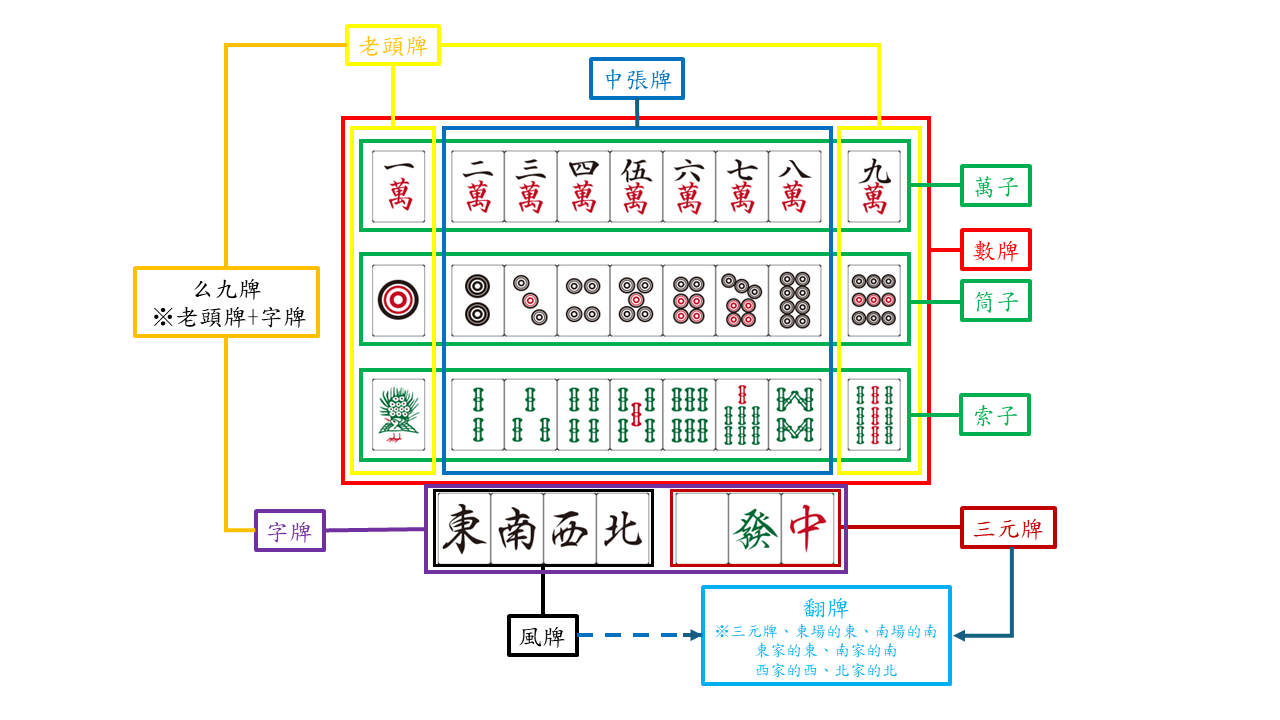
\includegraphics[width=1.0\textwidth]{牌種類.png}
        \end{figure}
    \item[3] 骰子
    \item[] 骰子使用2個六面骰。骰子合計的值稱為「出目」,對應方位如下:
    \begin{itemize}
        \item[$\bullet$]「2, 6, 10」 下家
        \item[$\bullet$]「3, 7, 11」 對家
        \item[$\bullet$]「4, 8, 12」 上家
        \item[$\bullet$]「5, 9」 \hspace{0.5cm} 自家
    \end{itemize}
    \item[4] 點棒
    \begin{itemize}
        \item[(1)] 分數的移動使用點棒
        \item[(2)]一套點棒含10000點1根、5000點1根、1000點4根、500點1根、100點5根共25000點。每位選手初始持有一套點棒, 若點棒數量有誤,選手有義務於對局開始前提出。
    \end{itemize}
    \item[5] 自動牌桌
    \item[] 對局使用具自動升起牌牆功能的麻將桌, 對局開始前應確認自動牌桌之功能是否正常。
    \item[6] 電梯線
    \item[] 牌牆升起的位置稱為電梯線
    \item[7] 裁判
    \item[] 對局中負責裁決的人稱為裁判。雖須絕對服從裁判之判決, 但至隔天為止皆可以書面方式提出異議。
    \item[8] 壁牌
    \item[] 碼好碼齊狀態的牌稱為壁牌
    \item[9] 墩
    \item[] 牌牆上下兩張為一組的單位稱為墩
    \item[10] 開門
    \item[] 每局開始時, 從牌牆中取配牌並開啟缺口的行為稱為開門。開門位置規定如下:
    \begin{itemize}
        \item [(1)] 以出目所指定方位之牌牆為開門對象
        \item[(2)] 自該牌牆面對桌子中央的左側數起, 留下出目數量的墩
    \end{itemize}
    \item[11] 王牌
    \begin{itemize}
        \item[(1)] 從開門位置順時針數起留下的共14張牌稱為王牌
        \item[(2)] 每當進行槓牌時, 將當前作為海底牌的牌補充進王牌中
        \item[(3)] 王牌中自順時針數起的前4張牌稱為嶺上牌
        \item[(4)] 嶺上牌的取得順序為 第一墩上層→第一墩下層→第二墩上層→第二墩下層
    \end{itemize}
    \item[12] 牌河
    \item[] 排列捨牌處稱為牌河
    \item[13] 海底牌
    \item[] 牌正前方最後的那張可摸之牌稱為海底牌
    \item[14] 河底牌
    \item[] 一局中切出的最後一張捨牌稱為河底牌
    \item[15] 手番
    \item[] 從摸牌或副露開始,到切牌為止的期間稱為手番
    \item[16] 牌的組合
    \item[] 牌的組合與稱呼規定如下:
        \begin{figure}[H]
        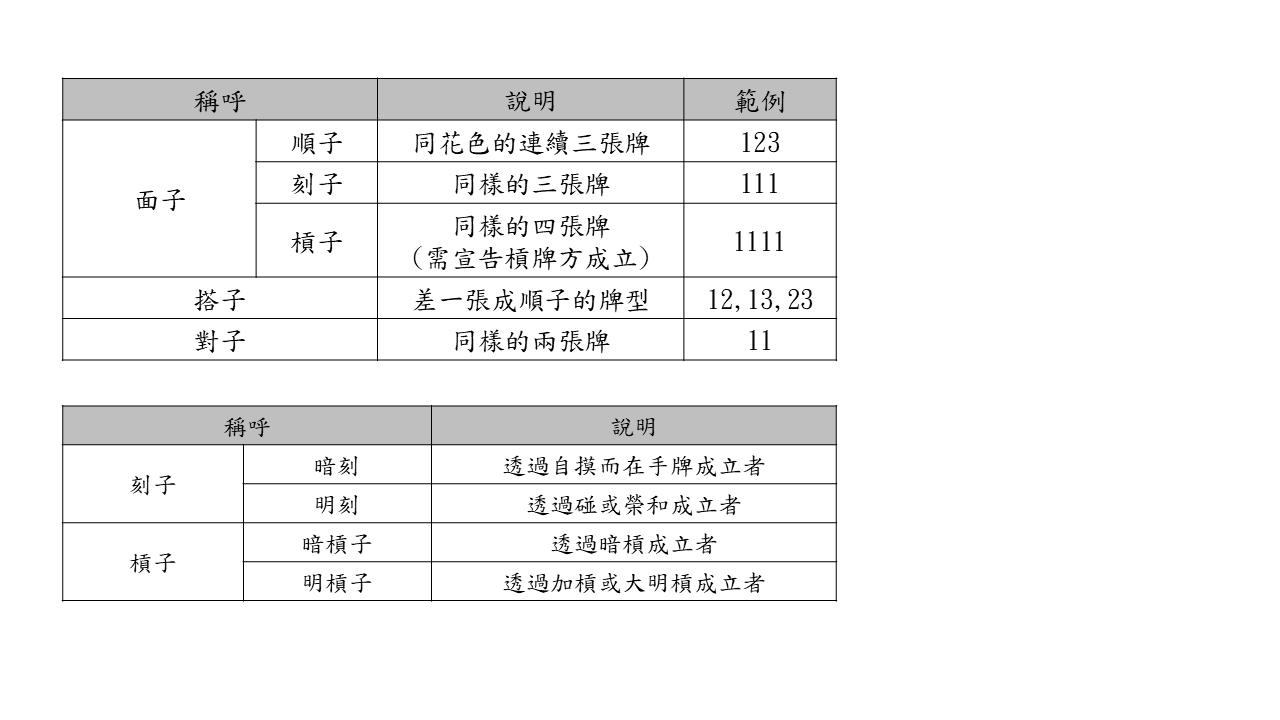
\includegraphics[width=0.8\textwidth]{牌組合.png}
        \end{figure}
    \item[17] 配牌
    \item[] 親家切出第一打前各家的手牌稱為配牌
    \item[18] 手牌
    \item[] 除自摸牌、嶺上自摸牌、副露牌之外,屬於自己的牌稱為手牌
    \item[19] 倒牌
    \item[] 將手牌全部正面朝上公開展示的行為稱為倒牌
    \item[20] 副露牌
    \item[] 因副露而亮出的面子,以及因加槓成立的明槓子、暗槓子,通稱為副露牌
    \item[21] 門前清
    \item[] 沒有任何副露的狀態稱為門前清
    \item[22] 家
        \begin{itemize}
            \item[(1)] 對局開始時的親家稱為起家
            \item[(2)] 從親家開始順時針分別稱為東家、南家、西家、北家
            \item[(3)] 東家也稱為莊家
            \item[(4)] 東家以外的三人稱為閒家
            \item[(5)] 自己也稱為自家
            \item[(6)] 自己以外的三人稱為他家
            \item[(7)] 左邊座位的人稱為上家、正面座位稱為對家、右邊座位稱為下家
        \end{itemize}
    \item[23] 寶牌
        \begin{itemize}
            \item[(1)] 面對王牌末尾席位的人,要將第1張嶺上牌移到第2張嶺上牌旁
            \item[(2)] 隨後,將王牌末尾數來第3墩上層的牌翻開。這張牌稱為寶牌指示牌
            \item[(3)] 根據寶牌指示牌,寶牌規定如下:
            \begin{itemize}
                \item[$\bullet$] 數牌:同花色依1→2→ \dots →8 →9 →1的順序之下一張
                \item[$\bullet$] 風牌:依東→南→西→北→東的順序之下一張
                \item[$\bullet$] 三元牌:依白→發→中→白的順序之下一張
            \end{itemize}
            \item[(4)] 和牌時,手牌中每有一張寶牌多加算一翻(包括和了牌)
            \item[(5)] 每次有槓牌時寶牌就會增加。第1次槓牌時,將當前顯示的寶牌指示牌鄰側(與王牌末尾相反方向)的牌翻開,這張成為新寶牌指示牌。此後以此類推。
            \item[(6)] 所有寶牌指示牌皆由面對該牌席位的人負責翻開
            \item[(7)] 立直後的和了可加算裏寶牌。當前顯示的寶牌指示牌之下層牌即為裏寶牌指示牌
            \item[(8)] 每套競技用牌中皆有赤五萬、赤五筒、赤五索各1張,這些牌稱為赤寶牌。赤寶牌視為寶牌
            \item[(9)] 所有寶牌皆不得因任何理由放棄
        \end{itemize}
    \item[24] 暴露牌
    \item[] 原本不該公開的牌不小心讓他人看見,稱為暴露牌。暴露牌必須向全員公開,並放回原位繼續對局
\end{itemize}
\section*{第三章 \ 競技的進行}
\end{document}